\section{Run a Single Instance of a Code and Load the Outputs}
The simplest exercise that can be performed is to run the driven code (\textbf{AnalyticBateman}  in our example), loading the results of a single run into RAVEN, printing and plotting some variables.
\\ As detailed in the RAVEN user manual (~\cite{RAVENuserManual}-Chapters ``DataObjects''  and ``Databases'') and in Chapter~/ref{sub:EntitiesAndFlow} RAVEN uses two classes of objects to store the data coming from a driven code (outputs):
\begin{itemize}
  \item \textbf{DataObjects}: The DataObjects represent the preferred way to transfer the information coming from a 
   Model (the driven code, in this case) to all the other RAVEN systems (e.g. Out-Stream system, Reduced Order Modeling
   component, etc.). 
  \item \textbf{Databases}.
\end{itemize}

As esaly inferable from the user manual (~\cite{RAVENuserManual}-Chapter ``OutStream''), the DataObjects can be exported into a CSV file and plotted (2-D and 3-D plots) linking them into the OutStream system.
\\ The following subsections report examples on how to use these systems running a single instance of the driven code.
\subsection{Single Run using the OutStream system for printing and create basic plots}
\label{sub:SingleRunBasicPlots}
 In this Section, the user can learn how to use RAVEN to run a single instance of a driven code, plotting and printing the 
 results.
 \\ The goal of this Section is to learn how to:
 \begin{enumerate}
   \item Set up a simple RAVEN input for running a driven code;
   \item Load the output of the code into the RAVEN DataObjects system;
   \item Print out what contained in the DataObjects;
   \item Generate basic plots of the code results.
\end{enumerate}  
In order to accomplish these tasks, the following RAVEN \textbf{Entities} (XML blocks in the input files) are needed:
 \begin{enumerate}
   \item \textbf{\textit{RunInfo}}:
\begin{lstlisting}[style=XML,morekeywords={arg,extension,pauseAtEnd,overwrite}]
    <RunInfo>
      <Sequence>Single, write-History</Sequence>
      <WorkingDir>SectionVI.I</WorkingDir>
      <batchSize>1</batchSize>
    </RunInfo>   
\end{lstlisting}   
   As reported in Section~\ref{sub:EntitiesAndFlow}, the \textit{RunInfo} \textbf{Entity} is intended to set up the analysis 
   that the user wants to perform. In this specific case, two steps (\xmlNode{Sequence}) are going to be sequentially run 
   using a single processor (\xmlNode{batchSize}).
   
   \item \textbf{\textit{Files}}:
\begin{lstlisting}[style=XML,morekeywords={arg,extension,pauseAtEnd,overwrite}]
  <Files>
    <Input name="referenceInput.xml" type="input">referenceInput.xml</Input>
  </Files>
\end{lstlisting}
   Since the driven code uses a single input file, in this Section the original input is placed. As described in the user manual~\cite{}
   the attribute  \xmlAttr{name} represents the alias that is going to be used in all the other input blocks in order to 
   refer to this file.
   \item \textbf{\textit{Models}}:
\begin{lstlisting}[style=XML,morekeywords={arg,extension,pauseAtEnd,overwrite}]
   <Models>
      <Code name="testModel" subType="GenericCode">
        <executable>
      ../physicalCode/analyticalbateman/AnalyticalDplMain.py
        </executable>
        <clargs arg="python" type="prepend"/>
        <clargs arg="" extension=".xml" type="input"/>
        <clargs arg="" extension=".csv" type="output"/>
        <prepend>python</prepend>
      </Code>
    <Models>
\end{lstlisting}
  Since the driven code already dumps its outputs in CSV format, there is no need to create
  an ad-hoc code interface and the GenericCode interface can be directly used. In additiom, since the \textbf{AnalyticBateman} code
  is written in \texttt{Python}, it is necessary to specify that the code needs to be run pre-pending the expression ``\texttt{Python}''. 
   \item \textbf{\textit{DataObjects}}:
\begin{lstlisting}[style=XML,morekeywords={arg,extension,pauseAtEnd,overwrite}]
  <DataObjects>
    <PointSet name="pointValues">
      <Input>InputPlaceHolder</Input>
      <Output>A,B,C,D</Output>
    </PointSet>
    <HistorySet name="history">
        <Input>InputPlaceHolder</Input>
        <Output>A,B,C,D,time</Output>
    </HistorySet>
  </DataObjects>
\end{lstlisting}
  Int this block, two \textit{DataObjects} are defined: 1) PointSet named ``pointValues'', 2) HistorySet named ``history''.
  Note that a special keyword is inputted in the \xmlNode{Input} node. This keyword is used when a \textit{DataObjects}  \textbf{Entity} needs to be constructed without any linking with respect to the input space. Indeed, in 
  this case, the model input space is not perturbed though a sampling strategies; the code is executed through the original
   input file   (``referenceInput.xml''). In the \xmlNode{Output} node all the requested variables are inputted.
   \item \textbf{\textit{OutStreams}}:   
\begin{lstlisting}[style=XML,morekeywords={arg,extension,pauseAtEnd,overwrite}]
  <OutStreams>
    <Print name="pointValues">
      <type>csv</type>
      <source>pointValues</source>
    </Print>
    <Print name="history">
        <type>csv</type>
        <source>history</source>
    </Print>
    <Plot dim="2" name="historyPlot" overwrite="false" verbosity="debug">
        <plotSettings>
            <plot>
                <type>line</type>
                <x>history|Output|time</x>
                <y>history|Output|A</y>
                <color>blue</color>
            </plot>
            <plot>
                <type>line</type>
                <x>history|Output|time</x>
                <y>history|Output|B</y>
                <color>red</color>
            </plot>
            <plot>
                <type>line</type>
                <x>history|Output|time</x>
                <y>history|Output|C</y>
                <color>yellow</color>
            </plot>
            <plot>
                <type>line</type>
                <x>history|Output|time</x>
                <y>history|Output|D</y>
                <color>black</color>
            </plot>
            <xlabel>time (s)</xlabel>
            <ylabel>evolution (kg)</ylabel>
        </plotSettings>
        <actions>
            <how>png,screen</how>
            <title>
                <text> </text>
            </title>
        </actions>
    </Plot>
  </OutStreams>
\end{lstlisting}
  In this block, both the Out-Stream types are constructed: 
  \begin{itemize}
    \item \textit{Print}: 
     \begin{itemize}
       \item named ``pointValues'' connected with the \textit{DataObjects} \textbf{Entity} ``pointValues'' 
                (\xmlNode{source})
       \item named ``history'' connected with the \textit{DataObjects} \textbf{Entity} ``history'' (\xmlNode{source})          
     \end{itemize}         
      When this objects get used, all the information contained in the linked  \textit{DataObjects} are going 
    to be dumped in CSV files (\xmlNode{type}).
    \item \textit{Plot}: a single \xmlNode{Plot} \textbf{Entity} is defined, containing the line plots of the 4 output variables 
    ($A,B,C,D$) in the same figure. This object is going to generate a PNG file and an interactive Plot on 
    the screen.
  \end{itemize}   
   \item \textbf{\textit{Steps}}:   
\begin{lstlisting}[style=XML,morekeywords={arg,extension,pauseAtEnd,overwrite}]
  <Steps>
    <SingleRun name="Single">
      <Input   class="Files"                        type="input">referenceInput.xml</Input>
      <Model  class="Models"                    type="Code">testModel</Model>
      <Output class="DataObjects"            type="PointSet">pointValues</Output>
      <Output class="DataObjects"            type="HistorySet">history</Output>
      <Output class="OutStreams" type="Print">pointValues</Output>
    </SingleRun>
    <IOStep name="writeHistory" pauseAtEnd="True">
        <Input    class="DataObjects"            type="HistorySet">history</Input>
        <Output class="OutStreams" type="Print">history</Output>
        <Output class="OutStreams" type="Plot">historyPlot</Output>
    </IOStep>
  </Steps>
\end{lstlisting}
 %%%%%%%%%%%%%%%%%%%%%%%%%%%%%%%%%%%%%%%%%%%%%%%%%%%%%%%%%%
 %figure history
 \begin{figure}[h!]
  \centering
  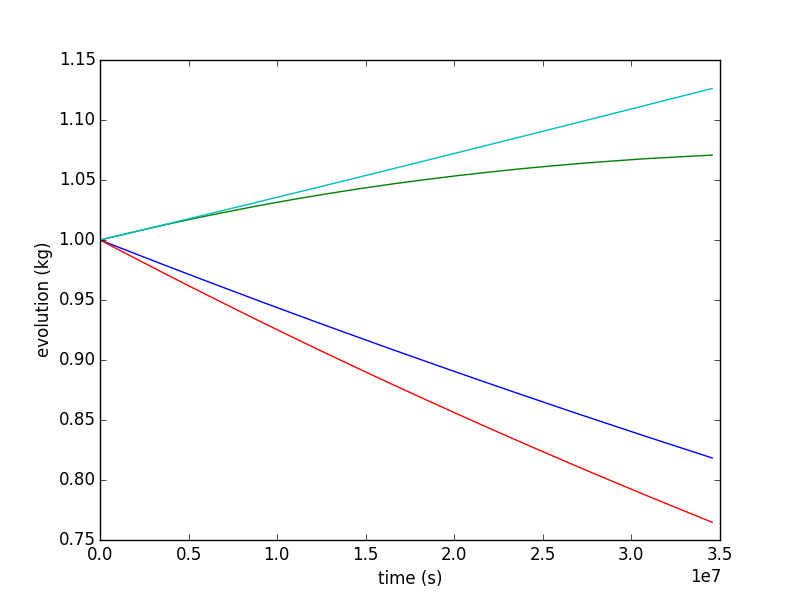
\includegraphics[scale=0.7]{pics/1-historyPlot_line-line-line-line.png}
  \caption{Plot of the history for variables $A,B,C,D$.}
  \label{fig:historyPlotLine}
 \end{figure}
 %%%%%%%%%%%%%%%%%%%%%%%%%%%%%%%%%%%%%%%%%%%%%%%%%%%%%%%%%%
   Finally, all the previously defined \textbf{Entities} can be combined in the \xmlNode{Steps} block. Thus, 
   two \xmlNode{Steps} have been inputted:
   \begin{itemize}
     \item \xmlNode{SingleRun} named ``Single'', used to run the single instance of the driven code and collect 
     the outputs in the two \textit{DataObjects}. In addition, it can be seen that an additional object has been  
     placed among the \xmlNode{Output}(s). Indeed, an  \textit{OutStreams} can be an \xmlNode{Output} in 
     any Step type (as long as the linked \textit{DataObjects} plays a whatever role in the Step)
     \item  \xmlNode{IOStep} named ``writeHistory'', used to 1) dump the ``history'' \textit{DataObjects} 
     \textbf{Entity} in a CSV file and 2) plot the data in the PNG file and on the screen.
   \end{itemize}
\end{enumerate} 
 Tables~\ref{historyVI.I} and \ref{pointValuesVI.I} show the results dumped by the OutStreams \textit{Print}.
 As previously mentioned, Figure~\ref{fig:historyPlotLine} reports the four plots (four variables) drawn in the same picture. 
 % table history set
\begin{table}[h!]
\centering
\caption{``history'' HistorySet CSV output file.}
\label{historyVI.I}
\begin{tabular}{|c|c|c|c|c|}
\hline
\textbf{A}                        & \textbf{C}                       & \textbf{B}                       & \textbf{D}                       & \textbf{time}                 \\ \hline
1                                 & 1                                & 1                                & 1                                & 0                             \\ \hline
0.983434738                       & 0.977851848                      & 1.010115067                      & 1.010131723                      & 2880000                       \\ \hline
0.967143884                       & 0.956202457                      & 1.019362317                      & 1.020361004                      & 5760000                       \\ \hline
0.951122893                       & 0.935040451                      & 1.027774063                      & 1.03067926                       & 8640000                       \\ \hline
0.941637969                       & 0.922572556                      & 1.032433141                      & 1.036909471                      & 10368000                      \\ \hline
0.932247632                       & 0.910273757                      & 1.036809334                      & 1.043167001                      & 12096000                      \\ \hline
0.922950939                       & 0.89814173                       & 1.040909121                      & 1.049450159                      & 13824000                      \\ \hline
0.913746955                       & 0.886174184                      & 1.044738857                      & 1.055757293                      & 15552000                      \\ \hline
0.904634757                       & 0.874368858                      & 1.048304784                      & 1.062086789                      & 17280000                      \\ \hline
0.886682065                       & 0.851235987                      & 1.054669586                      & 1.074806592                      & 20736000                      \\ \hline
0.869085647                       & 0.828725659                      & 1.060051155                      & 1.087597391                      & 24192000                      \\ \hline
\multicolumn{1}{|l|}{0.851838435} & \multicolumn{1}{l|}{0.806820897} & \multicolumn{1}{l|}{1.064495355} & \multicolumn{1}{l|}{1.100447571} & \multicolumn{1}{l|}{27648000} \\ \hline
\multicolumn{1}{|l|}{0.834933498} & \multicolumn{1}{l|}{0.785505192} & \multicolumn{1}{l|}{1.068046343} & \multicolumn{1}{l|}{1.113346061} & \multicolumn{1}{l|}{31104000} \\ \hline
\multicolumn{1}{|l|}{0.818364044} & \multicolumn{1}{l|}{0.764762489} & \multicolumn{1}{l|}{1.070746628} & \multicolumn{1}{l|}{1.126282318} & \multicolumn{1}{l|}{34560000} \\ \hline
\end{tabular}
\end{table} 
% table point set
\begin{table}[h!]
\centering
\caption{``pointValues'' PointSet CSV output file.}
\label{pointValuesVI.I}
\begin{tabular}{|c|c|c|c|c|}
\hline
\textbf{InputPlaceHolder} & \textbf{A}    & \textbf{C}     & \textbf{B}    & \textbf{D}    \\ \hline
0.0                       & 0.81836404385 & 0.764762489077 & 1.07074662835 & 1.12628231792 \\ \hline
\end{tabular}
\end{table}


\subsection{Single Run using the OutStream System to Sub-plot and Selectively print.}
This Section shows how to use RAVEN to create sub-plots (multiple plots in the same figure) and 
how to select only some variable from the \textit{DataObjects} in the \textit{Print} OutStream.
 \\ The goals of this Section are about learning how to:
 \begin{enumerate}
   \item Print out what contained in the DataObjects, selecting only few variables
   \item Generate sub-plots (multiple plots in the same figure) of the code results
\end{enumerate}  

To accomplish these tasks, the \textit{OutStreams} \textbf{Entity} in the input defined in the previous Section (~\ref{sub:SingleRunBasicPlots}) needs to be modified as follows:
\begin{enumerate}
   \item \textbf{\textit{Print}}:
   \begin{lstlisting}[style=XML,morekeywords={arg,extension,pauseAtEnd,overwrite}]
    <Print name="pointValues">
      <type>csv</type>
      <source>pointValues</source>
      <what>Output</what>
    </Print>
    <Print name="history">
        <type>csv</type>
        <source>history</source>
        <what>Output|A,Output|D</what>
    </Print>
   \end{lstlisting}   
   With respect to the \textit{Print} nodes defined in the previous Section (~\ref{sub:SingleRunBasicPlots}), it can
   be noticed that an additional node has been added: \xmlNode{what}. The \textit{Print} \textbf{Entity}  
   ``pointValues'' is going to extract and dump only the variables that are part of the Output space 
   ($A,B,C,D$ and not $InputPlaceHolder$).  The \textit{Print} \textbf{Entity} ``history'' is instead going to print 
   the Output space variables $A$ and $D$. 

   \item \textbf{\textit{Plot}}:
   \begin{lstlisting}[style=XML,morekeywords={arg,extension,pauseAtEnd,overwrite}]
    <Plot dim="2" name="historyPlot" overwrite="false" verbosity="debug">
        <plotSettings>
            <gridSpace>2 2</gridSpace>
            <plot>
                <type>line</type>
                <x>history|Output|time</x>
                <y>history|Output|A</y>
                <color>blue</color>
                <gridLocation>
                  <x>0</x>
                  <y>0</y>
                </gridLocation>
            </plot>
            <plot>
                <type>line</type>
                <x>history|Output|time</x>
                <y>history|Output|B</y>
                <color>red</color>
                <gridLocation>
                    <x>1</x>
                    <y>0</y>
                </gridLocation>
            </plot>
            <plot>
                <type>line</type>
                <x>history|Output|time</x>
                <y>history|Output|C</y>
                <color>yellow</color>
                <gridLocation>
                    <x>0</x>
                    <y>1</y>
                </gridLocation>
            </plot>
            <plot>
                <type>line</type>
                <x>history|Output|time</x>
                <y>history|Output|D</y>
                <color>black</color>
                <gridLocation>
                    <x>1</x>
                    <y>1</y>
                </gridLocation>
            </plot>
            <xlabel>time (s)</xlabel>
            <ylabel>evolution (kg)</ylabel>
        </plotSettings>
        <actions>
            <how>png,screen</how>
            <title>
                <text> </text>
            </title>
        </actions>
    </Plot>
\end{lstlisting}   
 Note that the  \textit{Plot} \textbf{Entity} does not differ much with respect to the one in 
 Section~\ref{sub:SingleRunBasicPlots}: 1) the additional sub-node \xmlNode{gridSpace}  has been added. 
 This node is needed to define how the figure needs to be partitioned (discretization of the grid). In this case
 a 2 by 2 grid is requested. 2) in each \xmlNode{plot} the node \xmlNode{gridLocation} is placed in 
 order to specify in which position the relative plot needs to be placed. For example, in the following grid 
 location, the relative plot is going to be placed at the bottom-right corner.
  \begin{lstlisting}[style=XML,morekeywords={arg,extension,pauseAtEnd,overwrite}]
   <gridLocation>
      <x>1</x>
      <y>1</y>
   </gridLocation>
   \end{lstlisting}   
 \end{enumerate}
The CSV tables generated by the \textit{Print} \textbf{Entities} are not reported, since the only differences with respect to Tables ~\ref{historyVI.I} and ~\ref{pointValuesVI.I} are related to the number of columns (variables)
dumped out. 
\\Figure~\ref{fig:historySubPlotLine} reports the four plots (four variables) drawn in the same picture. 
 %figure history sublots
 \begin{figure}[h!]
  \centering
  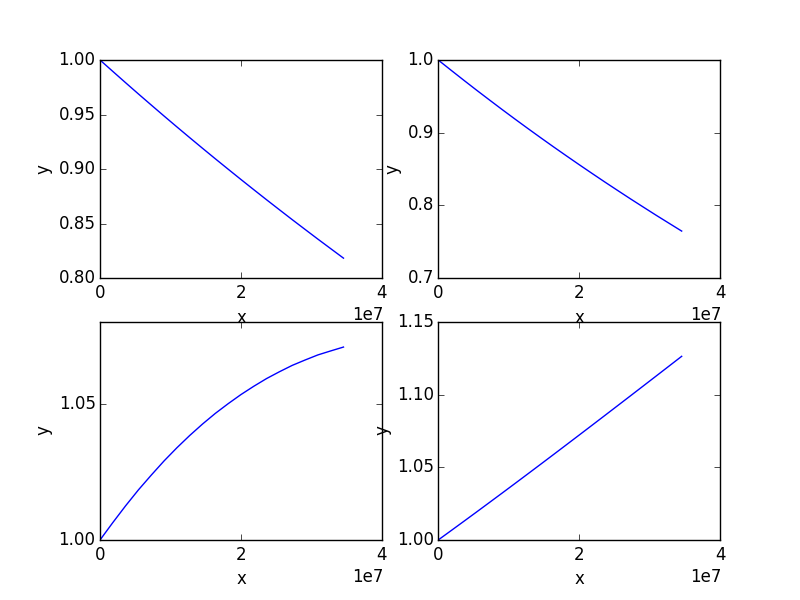
\includegraphics[scale=0.7]{pics/1-historyPlot_line-line-line-line-subPlots.png}
  \caption{Subplot of the history for variables $A,B,C,D$.}
  \label{fig:historySubPlotLine}
 \end{figure}

